\chapter{Introducción}
\label{ch:introduccion}

\begin{quote}
  En este capítulo se introduce el problema que se va a resolver en este proyecto, así como la motivación e impacto del mismo. Se presenta el concepto de Food Computing, el área de estudio en la que se engloba este trabajo. 
\end{quote}


\section{Motivación}
 
La nutrición es esencial para el desarrollo de la vida humana. Nuestros hábitos alimenticios tienen un impacto directo en nuestra salud, y por tanto, en nuestra calidad de vida. En los últimos años, se viene observando una tendencia al alza de enfermedades como la obesidad y la diabetes, a la par de un aumento de enfermedades cardiovasculares, todas ellas con estrecha relación con nuestra alimentación diaria~\cite{d2019obesity}. Esta involución nutricional tiene un origen complejo, en el que la interacción de factores culturales y socioeconómicos juegan un papel fundamental. Incluso en aquellas zonas donde la cultura gastronómica consta de características saludables (como es el caso de la dieta mediterránea), se observa una deriva nutricional hacia modelos menos recomendables y con impacto negativo en la salud. 

Estos problemas, unidos a la irrupción de la tecnología en la vida diaria, han sido uno de los puntos de partida del desarrollo de sistemas relacionados con la nutrición y el bienestar. 
Con las técnicas adecuadas y un correcto tratamiento y análisis, los datos generados por estos  sistemas se pueden utilizar para una mayor comprensión de esta área de estudio, especialmente desde un punto de vista dietético centrado en hábitos saludables.


\section{Concepto de Food Computing}

El uso de nuevas tecnologías para la interpretación y comprensión de grandes volúmenes de datos se aplica actualmente en múltiples áreas, entre las que se encuentra la nutrición. En ella, se trabaja con datos relativos a la alimentación, también conocidos como \textit{Food Data}.
%\textcolor{orange}{La relevancia que conlleva poder trabajar de forma automatizada con información alimenticia tiene un alto impacto en el análisis y estudio de la alimentación, especialmente desde un punto de vista dietético centrado en una alimentación saludable y vida sana. }% ya sea desde un punto de vista dietético centrado en una alimentación saludable y vida sana, o por la adecuación de éstas a las necesidades concretas por parte de quien las sigue.
En este contexto, se introduce el concepto de \textit{Food Computing}, el cual engloba la totalidad de técnicas y modalidades relativas a tareas de computación que utilizan datos alimenticios, de naturaleza heterogénea y procedentes de distintas fuentes de información~\cite{min2019survey}. Su finalidad es mejorar la calidad de vida de la población, así como entender de manera más profunda el comportamiento humano en lo que a esta área concierne. 

\begin{figure}[H]
    \centering
    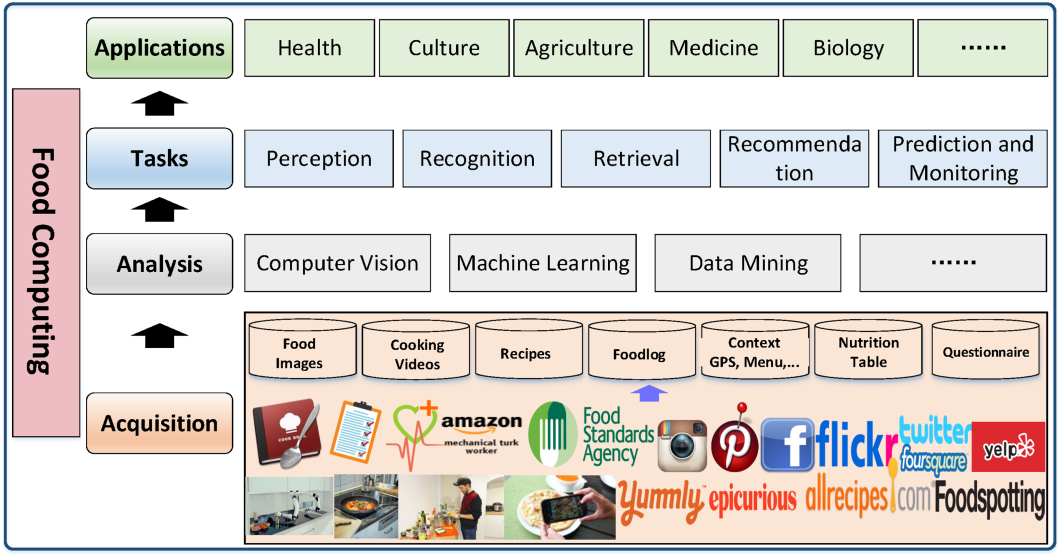
\includegraphics[width=1.0\textwidth]{imagenes/food_computing_1.png}
    \caption{Food Computing}
    \label{fig:food_computing_1}
\end{figure}

En términos generales, las tareas llevadas a cabo dentro del cuadro del Food Computing se caracterizan por partir de un procedimiento de extracción de información, el cual deriva en el desarrollo de herramientas cuyas tareas se pueden englobar en labores de reconocimiento de imágenes, percepción, recomendación, predicción y recuperación de información. De estas tareas destaca especialmente el aprendizaje predictivo, por su papel fundamental en la resolución de problemas en Food Computing~\cite{min2019survey}. Es tal su relevancia que no solo se corresponde con una de las tareas fundamentales abordadas en este ámbito, sino que también cobra protagonismo en las otras mencionadas, bien ocupándose de funcionalidades muy específicas, bien a nivel global, con el fin de dotar de \textit{inteligencia} a la solución (p.ej., capacidad de decisión, identificación de entidades, detección de comportamientos anómalos o previsión de comportamientos futuros que pueda tener un sistema). 

La aplicación de estas tareas no solo afecta a la nutrición sino que también utilizan conocimiento específico de otras áreas para abordar problemas relacionados con la alimentación tales como la medicina, la biología, la gastronomía la agronomía o la cultura. En la Figura \ref{fig:food_computing_1} se muestra un esquema simplificado de todo lo que engloba el concepto de Food Computing~\cite{min2019survey}. 
En ella se aprecia cómo las técnicas predictivas tienen una gran presencia en este campo, ya que además de formar una de las tareas principales, también se encuentran de forma intrínseca en las labores de análisis (Visión por Computador, Aprendizaje Automático y Minería de textos entre otras).

Uno de las mayores desafíos a abordar cuando se trabaja con problemas de Food Computing es la dificultad intrínseca que conlleva el tratamiento de la información. Con ello, no solo nos referimos a la gran cantidad de datos que se generan hoy en día dentro de este contexto, sino también a la dificultad añadida de trabajar con su distinta naturaleza y origen. Abordar un problema de Food Computing suele llevar asociado la necesidad de trabajar de forma simultánea con datos de distintos contextos, como pueden ser la tecnología de alimentos, la nutrición y las redes sociales. %Trabajar de forma conjunta con estos datos es, 
En una primera instancia esto puede resultar inviable, ya que se tratan de fuentes de información muy heterogéneas entre sí, las cuales no se encuentran agregadas y requieren un tratamiento previo que permita poder trabajar con todos los datos de forma simultánea. En esta línea, se pueden utilizar modelos predictivos de lenguaje para identificar elementos equivalentes que se encuentren en dos o más conjuntos de datos, y así poder integrar distintas fuentes y trabajar con ellas como si de una única colección de datos se tratase.

\section{Nuestro problema a resolver}

Tal y como se ha introducido previamente, en el mundo de la alimentación es difícil trabajar con todos los datos requeridos, puesto que las fuentes de información no suelen proporcionarlos de manera directa. Un ejemplo claro son las páginas web de recetas, fuentes de información protagonistas en este ámbito. Normalmente, trabajar con estas recetas desde un punto de vista nutricional requiere de un uso conjunto de sus ingredientes con una base de datos de composición de alimentos para así poder extrapolar su información nutricional. 

Para trabajar de forma conjunta con ambas fuentes de información se requiere un proceso intermedio que haga de intermediario y facilite el tratamiento de datos de distinta naturaleza y origen. Esta idea se refleja en la Figura \ref{fig:heterogeneos_}, donde se puede ver cómo la información alimenticia se nutre de múltiples fuentes de información, dando lugar a un único elemento que se ha denominado en dicha figura como \textit{item food}, que representa al objeto fusionado que se aspira a obtener. Esta dificultad no es específica de Food Computing, sino que se encuentra presente en cualquier área de estudio que combine información de distinto tipo y necesite trabajar con ella de forma conjunta, como puede ser por ejemplo, en el área de medicina al trabajar con datos biomédicos de usuarios y bases de datos de conocimiento o en el área legal, donde fuentes de conocimiento legislativo experto se combinan con sucesos o eventos concretos. 

\begin{figure}[H]
    \centering
    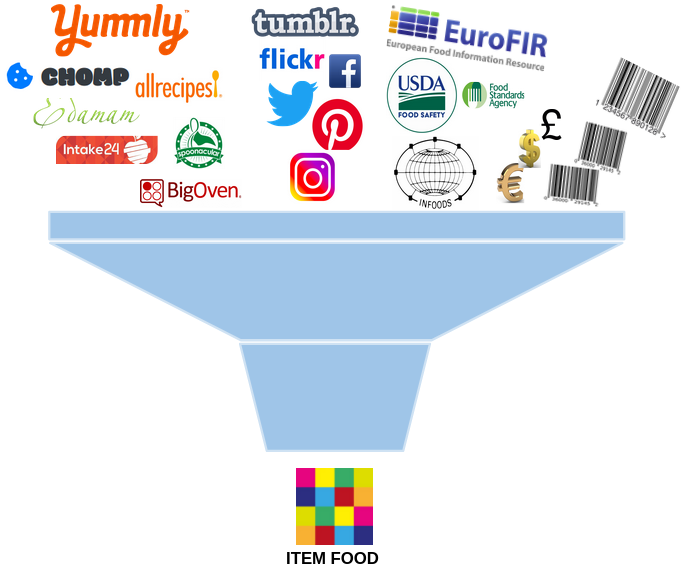
\includegraphics[width=0.8\textwidth]{imagenes/IMAGE.png}
    \caption{Datos heterogéneos en Food Computing}
    \label{fig:heterogeneos_}
\end{figure}

En este trabajo, se desarrolla una herramienta que permite fusionar información heterogénea procedente de diferentes fuentes de datos con el fin de trabajar con ellas simultáneamente. Para ello, se identificarán elementos equivalentes entre las distintas fuentes, para así poder integrarlos y utilizarlos de manera combinada. El problema de identificación de términos equivalentes se puede abordar desde un punto de vista predictivo a partir de varios enfoques. En nuestro caso, lo abordaremos desde la perspectiva del Procesamiento de Lenguaje Natural, utilizando un modelo predictivo de Word Embedding (Word2vec) entrenado con textos de recetas para aprender representaciones de palabras. Con el fin de detectar correspondencias entre los datos, se llevará a cabo un procedimiento de mapeo que utilice dichas representaciones para medir la similitud entre elementos.

%Para ello, se consideran medidas de distancia que tienen en cuenta tanto las características sintácticas del texto, como la información semántica capturada por el modelo. Estas medidas se han estudiado desde las perspectivas clásica y difusa con el objetivo de determinar qué enfoque es el más adecuado para nuestro problema. 
%que nos permita capturar la información semántica de los textos a la hora de obtener su representación. 

Se mostrará su funcionamiento dentro de un sistema que permita su uso para abordar algún problema concreto con los datos ya combinados. En nuestro caso, lo haremos con una aplicación dentro del área de la nutrición, desarrollando un sistema de adaptación de recetas a restricciones alimenticias de usuario, como pueden ser intolerancias a algún alimento, alergias, o incluso restricciones derivadas de dietas como puede ser la vegetariana o la vegana. Este sistema permitirá recomendar, en base a dichas restricciones, posibles variaciones de recetas a través de modificaciones de sus ingredientes. La adaptación de recetas se llevará a cabo gracias al uso previo de la herramienta de fusión de información heterogénea, la cual permitirá combinar recetas de cocina con la información nutricional de sus ingredientes para poder detectar las restricciones alimenticias que deban solventarse.

De las tareas de Food Computing mencionadas anteriormente, con este problema se aborda principalmente un problema de \textbf{Predicción} para la creación de un modelo de lenguaje. Se lleva a cabo el entrenamiento de un modelo predictivo de tratamiento del lenguaje basado en un Word Embedding entrenado sobre un conjunto de recetas que permita identificar términos alimenticios. Por otra parte, también se engloba en otras tareas de Food Computing: sin seguir las estructuras tradicionales y estandarizadas de sistemas basados en recomendación, proporciona opciones de recetas personalizadas a unas preferencias de usuario concretas, resolviendo así un problema en el ámbito de la \textbf{Recomendación} en Food Computing. Problemas de \textbf{Recuperación} e \textbf{Identificación} también se encuentran intrínsecos en este trabajo, puesto que se llevan a cabo tanto la obtención del corpus y fuentes de datos utilizadas para resolver este problema como una tarea de identificación de elementos alimenticios en distintas bases de datos.

\section{Objetivos}\label{sec:objetivos}

Para poder abordar el diseño e implementación de un sistema que permita poner solución al problema descrito en el apartado anterior, se ha marcado como objetivo principal el estudio, diseño e implementación de técnicas predictivas para resolver un problema de Procesamiento de Lenguaje Natural. De este objetivo general se derivan los siguientes objetivos específicos:

\begin{enumerate}
    \item\textit{Identificar los elementos a los que representan los datos que intervienen en el problema}: asignar una representación interna a los datos a través de sus descripciones textuales, con la que poder detectar equivalencias para así realizar la agregación entre las fuentes de datos.

    \item\textit{Fusionar información heterogénea}: desarrollar una herramienta que permita agregar datos de distinta naturaleza y procedencia que necesiten ser tratados de manera conjunta a la hora de abordar algún problema concreto.
    
    \item\textit{Mostrar la eficacia y el alcance de la herramienta desarrollada}: argumentar la utilidad de la herramienta con un problema real y de interés actual: la sustitución de elementos por otros similares mediante el modelo predictivo y las representaciones textuales que genera.
    
\end{enumerate}

\section{Contenido de la memoria en relación a los objetivos}

La memoria se ha redactado en función de los tres grandes pilares en los que se basa este trabajo, los cuales hacen referencia a los tres objetivos específicos detallados en este primer capítulo. En el Capítulo 2 se especifican los requisitos y la planificación por actividades llevada a cabo, las cuales están directamente ligadas a los objetivos. En el Capítulo 3 se exponen los antecedentes que preceden a este trabajo; se profundiza en el concepto de \textit{Food Computing} así como en la revisión bibliográfica de las técnicas de predicción en los problemas abordados en este campo. En el Capítulo 4 se describe de forma general la arquitectura del sistema diseñado para abordar el problema. Se especifican los tres pilares en los que se basa el proyecto como módulos que permiten construir la solución. Estos módulos se relatan de forma detallada en los Capítulos 5, 6 y 7, abarcando el diseño y la implementación llevada a cabo para cada uno de ellos. En el Capítulo 8 se detalla la experimentación y resultados obtenidos en cada uno de los módulos. Por último, en el Capítulo 9, se exponen todas las conclusiones obtenidas a lo largo del trabajo, así como las posibles líneas que se podrían seguir explorando a partir de este trabajo. 

\newpage